\chapter{Présentation de l'entreprise}

\section{VideoStitch}
\subsection{Présentation générale}
\begin{wrapfigure}[5]{r}{7cm}
  \centering
  
\includegraphics[width=6cm]{images/videostitch.jpg}
  \caption{Logo de VideoStitch}
\end{wrapfigure}
VideoStitch est une entreprise française d'édition de logiciels, qui conçoit et 
vend des logiciels de capture, de montage, de montage, de diffusion et de lecture 
de vidéos panoramiques à 360\degree. Elle s'intéresse par extension au marché de 
la réalité virtuelle.
Son site internet est à l'adresse suivante : \url{http://www.video-stitch.com/}.\\
C'est une Société à Actions Simplifiées (SAS) basée sur Paris, qui emploie moins
d'une dizaine de personnes actuellement. La plupart ayant été embauchés il y a 
quelques mois, c'est une société en forte croissance salariale. 
Nicolas Burtey en est le président.

\subsection{Historique}
VideoStitch a été fondée par ce même Nicolas Burtey en janvier 2012.\\
Photographe diplômé de l'Ecole Lumière, s'étant fait connaître par la photo panoramique 
et la photo fish-eye, M. Burtey évolue par la suite dans le domaine de la vidéo panoramique.\\
\begin{wrapfigure}[5]{l}{6cm}
  \centering
  
\includegraphics[width=5cm]{images/loopin.png}
  \caption{Logo de Loop'In}
\end{wrapfigure}
Il crée sa société de production vidéo, Loop'In, avec laquelle il réalise une 
certain nombre de vidéos panoramiques à 360\degree pour des boites de production (publicité essentiellement). 
Des exemples de ces vidéos sont disponibles à cette adresse : \url{http://www.loop-in.com/galerie/}.
La vidéo panoramique, étant alors un procédé très jeune encore inconnu du grand public, est 
lente et difficile à réaliser: beaucoup de tâches doivent être faites de manière 
manuelle et répétitive, avec des outils inadaptés car non prévus à cette utilisation.
Si la création de photos panoramiques et à 360\degree est aisée, il manque toutefois 
un logiciel complet et mature qui permetrait l'édition et le montage de vidéos paramiques.\\
\newline
M. Burtey décide alors de créer VideoStitch pour concevoir cet outil, un logiciel 
d'édition et de montage de vidéos panoramiques : VideoStitch Studio.\\
Quand ce logiciel atteint une version stable, en 2014, VideoStitch oriente alors 
ses efforts vers un nouveau logiciel, Vahana VR, permettant cette fois-ci une réalisation 
et une diffusion en direct de vidéos panoramiques à 360\degree.\\
\newline
Le but de la société est de permettre une réalisation aisée et de qualité de vidéos 
panoramiques à 360\degree, de la capture des images à la diffusion de la vidéo finale, 
en passant par sa réalisation complète.


\section{La vidéo 360}
\subsection{Du panorama à la vidéo 360}
Une image panoramique, ou panorama, est une superposition d'images qui sont assemblées
afin de composer une vue bien plus large que ne le permet une image seule. La figure~ 
\ref{RochesterNY} présente un exemple d'assemblage d'un panorama.\\
Concrètement, avec un appareil photograhique, cela consiste à prendre plusieurs vues
successives en tournant l'appareil autour d'un axe entre deux clichés. 
Les photos obtenues forment ainsi une série d'un même sujet et doivent pouvoir chevaucher 
pour être ensuite assemblées en une image panoramique. 
Cet assemblage peut être réalisé avec directement par l'appareil, c'est le cas des 
téléphones portables, ou par un logiciel spécialisé, comme Photoshop\cite{photomerge} 
ou PTgui\cite{PTgui}.
\begin{figure}
  \centering
  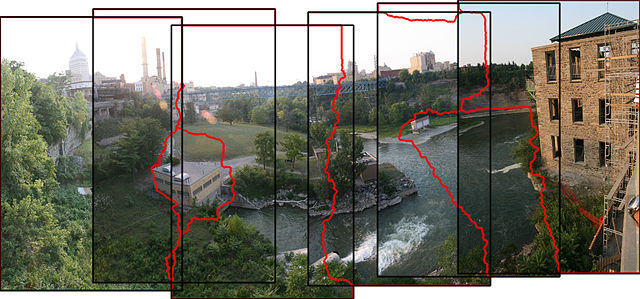
\includegraphics[width=12cm]{images/RochesterNY.jpg}
  \caption{Exemple d'assemblage de panorama avec détection des zones de chevauchement\cite{RochesterNY}}
  \label{RochesterNY}
\end{figure}
\newline
La vidéo panoramique consiste à filmer avec plusieurs caméras en même temps, chacune
capturant une partie du panorama, pour assembler les images capturées en une seule
vidéo par le même princique que la photo panoramique.\\
Avec suffisament de caméras, il est possible de couvrir un angle de prise de vue 
de 360\degree à l'horizontale et de 180\degree à la verticale. Le panorama créé
forme alors une sphère virtuelle, comme le montre la figure~\ref{rig-sphère}. 
C'est ce qu'on appelle la vidéo 360.
\begin{figure}
  \centering
  figure exemple, rig avec sphère virtuelle
\end{figure}
\newline
Cependant, comme le montre la figure~\ref{RochesterNY}, un panorama reste une image
$-$ ou une vidéo $-$, c'est-à-dire une matrice plane consistuée de pixels\footnote{Pour
 \enquote{picture element}}. Or une vidéo 360 représentant une sphère virtuelle, ou
plutôt sa surface, elle sera nécessairement une \emph{projection} de cette sphère, 
c'est-à-dire une correspondance mathématique entre cette surface en 3 dimensions 
et cette vidéo plane\cite{projection-cartographique}.\\
Dans la vidéo 360, la projection la plus utilisée est la projection équirectangulaire\cite{what-is-equirectangular}.
Un exemple en est le planisphère terrestre, où après une projection cylindrique équirectangulaire
sur la figure~\ref{projection-cylindrique} le plan est déroulé pour obtenir le 
planisphère de la figure~\ref{planisphère}.
\begin{figure}
  \centering
  \begin{minipage}{0.4\textwidth}
    \centering
    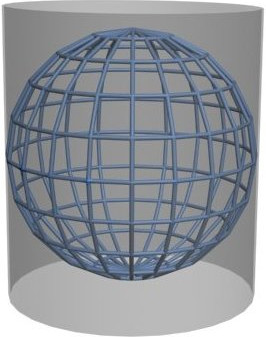
\includegraphics[width=4cm]{images/Projection-cylindrique.jpg}
    \captionof{figure}{Schéma d'une projection équirectangulaire}
    \label{projection-cylindrique}
  \end{minipage}%
  \begin{minipage}{0.6\textwidth}
    \centering
    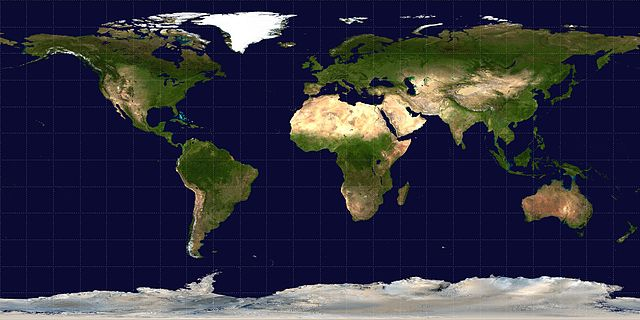
\includegraphics[width=9cm]{images/Equirectangular-projection.jpg}
    \captionof{figure}{Projection équirectangulaire de la Terre}
    \label{planisphère}
  \end{minipage}
\end{figure}
\newline
Un lecteur vidéo 360 est alors nécessaire pour lire correctement la vidéo~: 
il va reconstruire la sphère, pour y projetter le panorama et y placer le
spectateur au centre de cette sphère. Dès lors, le spectateur peut déplacer le 
regard tout autour de lui pour embrasser le panorama : on entre dans le champs de 
la réalité virtuelle\footnote{La réalité virtuelle est ici comprise dans son sens
  de \enquote{Simulation sensorielle immersive de la réalité}\cite{definition-rv}}.

\subsection{Le marché de la vidéo 360}
Si les années 2000 ont vu la démocratisation des appareils photographiques numériques,
les années 2010 voient l'émergence des caméras numériques Haute 
Définition\footnote{Définition d'image de 1920x1080 pixels} peu chères, comme les GoPro,
et d'écrans 4K\footnote{Définition d'image de 4096x2160 pixels}. De plus les capacités
informatiques grand public permettent désormais de stocker et traiter plusieurs 
vidéos HD en même temps.\\
Dès lors la vidéo 360 peut se développer, son coût technique
étant accessible, et le marché, bien qu'encore restreint et peu visible du public,
est un plein développement et présente déjà de très nombreux concurrents. Jaunt,
entreprise américaine créée en mai 2013 a, par exemple, déjà levé 35 millions
de dollars de fonds d'investissements\cite{jaunt-fundings}.\\
Les grandes entreprises comme Facebook\cite{facebook-vr}, Samsung\cite{samsung-vr}, 
Microsoft\cite{microsoft-vr} ou Google\cite{google-vr} suivent de
très près ce marché, notamment pour concevoir des produits de réalité virtuelle 
ou de réalité augmentée.

\section{Produits et stratégies de l'entreprise}
% Analyse de l'avenir des marchés, stratégies de positionnement et d'investissement, ambitions
